% AI Finance 2 — A. 공개 거래 데이터 지도 (Beamer, metropolis)
% 빌드: xelatex AI_Finance_2_A_데이터지도.tex  (두 번)
\documentclass[aspectratio=169,10pt]{beamer}
% 공통 스타일 (metropolis, 한글, 색, 표, 그림)
\usetheme[progressbar=frametitle,numbering=fraction,block=fill]{metropolis}

\usepackage{fontspec}
\usepackage[hangul]{kotex}
\setmainfont{Apple SD Gothic Neo}
\setsansfont{Apple SD Gothic Neo}[BoldFont={* Bold}]
\setmonofont{Menlo}[Scale=0.88]
\setmainhangulfont{Apple SD Gothic Neo}
\setsanshangulfont{Apple SD Gothic Neo}[BoldFont={* Bold}]
\setmonohangulfont{Apple SD Gothic Neo}

\usepackage{booktabs,tabularx,array,colortbl}
\usepackage{pgfplots}
\pgfplotsset{compat=1.18,/pgf/number format/1000 sep={\mathord{,}}}
\usepackage{tikz}
\usetikzlibrary{arrows.meta,positioning,shapes.misc}

% 색 (metropolis 기본과 맞춤)
\definecolor{ink}{HTML}{23373B}
\definecolor{accent}{HTML}{EB811B}
\definecolor{teal}{HTML}{14B03D}
\definecolor{blue}{HTML}{2B5EA7}
\definecolor{soft}{HTML}{F2F4F8}
\definecolor{muted}{HTML}{6B7785}
\setbeamercolor{alerted text}{fg=accent}
\setbeamercolor{block title}{bg=ink!12,fg=ink}
\setbeamercolor{block body}{bg=soft}

\newcommand{\src}[1]{{\scriptsize\color{muted}#1}}
\newcommand{\num}[1]{{\color{accent}\textbf{#1}}}
\newcommand{\tagbox}[2]{{\setlength{\fboxsep}{2.5pt}\colorbox{#1}{\textcolor{white}{\scriptsize\bfseries #2}}}}
\renewcommand{\arraystretch}{1.25}
\tikzset{card/.style={rectangle,rounded corners=4pt,draw=#1,line width=0.9pt,fill=#1!6,
               minimum width=6.6cm,minimum height=2.25cm,align=left,text width=6.2cm,inner sep=6pt},
  box/.style={rounded corners=3pt,draw=#1,fill=#1!8,line width=0.8pt,minimum width=4.2cm,minimum height=0.9cm,align=center,font=\small},
  arr/.style={-{Stealth[length=5pt]},line width=0.8pt,muted}}

% Claude 요청문·코드: \begin{Verbatim} … \end{Verbatim} (frame은 [fragile])
\usepackage{fvextra}
\fvset{breaklines=true,breakanywhere=true,breaksymbolleft={},fontsize=\scriptsize,frame=leftline,framerule=2pt,rulecolor=\color{accent},xleftmargin=4pt,framesep=6pt}


\title{공개 거래 데이터 지도}
\subtitle{AI Finance 2 · A — 어디서, 무엇을, 언제, 얼마나 가려서}
\date{2026년 12월 5일}

\begin{document}

\maketitle

% ─────────────────────────────────────────────
\begin{frame}{오늘의 역할}
\begin{columns}[T]
\begin{column}{0.47\textwidth}
\begin{block}{1일차 — 상품 문서}
JPMorgan이 낸 \textbf{424B2 공시} 1,859건\\[2pt]
글을 텍스트로 바꾸고, 검색하고, 뽑았다.
\end{block}
\end{column}
\begin{column}{0.47\textwidth}
\begin{alertblock}{2일차 — 시장 금리}
그 상품의 가격을 정하는 \textbf{기준 금리}\\[2pt]
누구나 받을 수 있는 \textbf{공개 거래 데이터}로 확인한다.
\end{alertblock}
\end{column}
\end{columns}
\vspace{1.2em}
\begin{center}
\large 나는 JPMorgan 구조화상품 담당자다.\\[3pt]
\normalsize\color{muted} 오늘은 DB도 Azure도 없이 — VS Code, Claude Code, \texttt{uv}만.
\end{center}
\end{frame}

% ─────────────────────────────────────────────
\begin{frame}{지도 한 장: 네 곳}
\begin{tikzpicture}
\node[card=accent] (a) at (0,0) {\textbf{\large ① DTCC 스왑 공시}\\[2pt]
  \small 장외 스왑 \textbf{거래 한 건 한 건}\\
  \small 체결 약 \textbf{2분} 뒤 공개 · 익명\\
  \scriptsize\color{muted} 법(CFTC Part 43, SEC Reg SBSR)이 공개를 요구};
\node[card=blue] (b) at (7.2,0) {\textbf{\large ② NY Fed 기준금리}\\[2pt]
  \small \textbf{하루에 숫자 하나}: SOFR\\
  \small 다음 영업일 22:00(한국) 발표\\
  \scriptsize\color{muted} 국채 담보 하루짜리 레포 금리의 공식 산출 기관};
\node[card=teal] (c) at (0,-2.6) {\textbf{\large ③ 재무부 국채 금리}\\[2pt]
  \small \textbf{하루에 곡선 하나}: 1개월–30년\\
  \small 미국 장 마감 후 발표\\
  \scriptsize\color{muted} 시장 가격으로 만든 공식 수익률 곡선};
\node[card=ink] (d) at (7.2,-2.6) {\textbf{\large ④ TreasuryDirect 경매}\\[2pt]
  \small \textbf{경매 한 번에 한 행}\\
  \small 낙찰 금리 · 응찰 배율 · 발행액\\
  \scriptsize\color{muted} 새로 발행하는 국채의 경매 결과};
\end{tikzpicture}
\end{frame}

% ─────────────────────────────────────────────
\begin{frame}{무엇이 들어 있고, 무엇이 가려져 있나}
\small
\begin{tabularx}{\textwidth}{@{}l X X@{}}
\toprule
 & \textbf{들어 있는 것} & \textbf{가려진 것} \\
\midrule
\tagbox{accent}{① DTCC} & 체결 시각, 시작일·만기일, 원금, 통화, 고정금리, 기초금리 이름, 청산 여부, 거래 플랫폼 \src{(한 건에 항목 110개)} & \alert{거래 상대방 이름 없음}. 큰 거래는 원금에 상한(\texttt{250,000,000+}). 블록 거래는 늦게 공개 \\
\tagbox{blue}{② NY Fed} & SOFR, 거래량, 분포(1·25·75·99 백분위). EFFR·BGCR·TGCR·OBFR도 & 개별 거래 없음 (집계값) \\
\tagbox{teal}{③ 재무부} & 1개월–30년, 14개 만기의 수익률 & 개별 거래 없음 (모형으로 만든 곡선) \\
\tagbox{ink}{④ 경매} & 낙찰 금리, 응찰 배율, 발행액, 입찰자 유형별 배정 \src{(항목 187개)} & 누가 샀는지 없음 (유형별 집계) \\
\bottomrule
\end{tabularx}
\end{frame}

% ─────────────────────────────────────────────
\begin{frame}{언제 나오고, 얼마나 쌓여 있나}
\small
\begin{tabularx}{\textwidth}{@{}l X l l l@{}}
\toprule
 & \textbf{언제 (한국 시간)} & \textbf{쌓인 기간} & \textbf{크기} & \textbf{공식 API} \\
\midrule
\tagbox{accent}{① DTCC} & 거래 후 \num{약 2분} (블록 약 15분)\newline 하루치 파일은 \num{다음 날 09:15} & 약 1년 (2025-11-26–) & 평일 2만–3만 건 & \alert{아니오} \\
\tagbox{blue}{② NY Fed} & 다음 영업일 \num{22:00} (뉴욕 08:00) & 2018년 4월– & 하루 1줄 & 예 \\
\tagbox{teal}{③ 재무부} & 그날 미국 장 마감 후 & 1990년– & 하루 1줄 & 예 \\
\tagbox{ink}{④ 경매} & 경매 결과 발표 직후 & 수십 년치 & 하루 0–몇 건 & 예 \\
\bottomrule
\end{tabularx}
\vspace{0.8em}
\begin{alertblock}{토요일 아침 수업}
지금 미국은 금요일 저녁, 서울·도쿄는 토요일. \textbf{새 거래가 없다} — 공개 데이터도 시장 시간을 따른다.
\end{alertblock}
\end{frame}

% ─────────────────────────────────────────────
\begin{frame}[fragile]{받는 주소}
\footnotesize
\begin{tabularx}{\textwidth}{@{}l X@{}}
\toprule
\tagbox{accent}{① 최근 100건} & \texttt{pddata.dtcc.com/ppd/api/ticker/CFTC/RATES} \\
\tagbox{accent}{① 하루치 zip} & \texttt{kgc0418-tdw-data-0.s3.amazonaws.com/cftc/eod/}\\
 & \texttt{\quad CFTC\_CUMULATIVE\_RATES\_2026\_11\_25.zip} \\
\tagbox{blue}{② SOFR} & \texttt{markets.newyorkfed.org/api/rates/secured/sofr/last/5.json} \\
\tagbox{teal}{③ 국채 곡선} & \texttt{home.treasury.gov/resource-center/data-chart-center/interest-rates/}\\
 & \texttt{\quad pages/xml?data=daily\_treasury\_yield\_curve\&field\_tdr\_date\_value\_month=202611} \\
\tagbox{ink}{④ 경매} & \texttt{www.treasurydirect.gov/TA\_WS/securities/auctioned?format=json} \\
\bottomrule
\end{tabularx}
\vspace{0.6em}
\src{① DTCC는 공개 대시보드가 쓰는 주소다. 1분에 한 번 이하로 부르고, 많이 받을 때는 하루치 zip을 쓴다.}
\end{frame}

% ─────────────────────────────────────────────
\begin{frame}{1일차 SEC 공시 vs 오늘 DTCC 스왑 공시}
\begin{tabularx}{\textwidth}{@{}l X X@{}}
\toprule
 & \textbf{1일차: SEC 424B2} & \textbf{오늘: DTCC} \\
\midrule
누가 쓰나 & 발행사(JPMorgan)가 직접 & 거래 당사자가 신고 → DTCC가 공개 \\
단위 & 상품 설명서 한 건 (글) & 거래 한 건 (숫자 칸) \\
이름 & 발행사·상품명 그대로 & \alert{익명} — JPMorgan 거래만 골라낼 수 없다 \\
언제 & 발행할 때 & 체결 몇 분 뒤 \\
핵심 기술 & 텍스트 변환 · 검색 · 추출 & \alert{어떤 행을 걸러낼지} \\
\bottomrule
\end{tabularx}
\end{frame}

% ─────────────────────────────────────────────
\section{거래 한 건 읽기}

\begin{frame}{미국 달러 10년 SOFR 스왑 \src{\normalsize 2026-11-25, DTCC 하루치 파일}}
\small
\begin{columns}[T]
\begin{column}{0.56\textwidth}
\begin{tabularx}{\textwidth}{@{}l >{\ttfamily}X@{}}
\toprule
Action / Event type & NEWT / TRAD \\
Execution Timestamp & 2026-11-25T08:23:42Z \\
Effective → Expiration & 2026-12-16 → 2036-12-16 \\
Notional & 62,000,000 USD \\
Fixed rate-Leg 1 & \textcolor{accent}{\bfseries 0.044617} \\
UPI Underlier Name & USD-SOFR-OIS Compound \\
Cleared / Platform & I / TWSF \\
Block trade & FALSE \\
\bottomrule
\end{tabularx}
\end{column}
\begin{column}{0.40\textwidth}
\begin{block}{읽으면}
한국 시간 \textbf{17:23} 체결\\
3주 뒤 시작하는 \textbf{10년} 스왑\\
원금 \textbf{6,200만 달러}\\
고정 \num{4.4617\%} ↔ SOFR 복리\\
청산 예정, Tradeweb 플랫폼
\end{block}
\src{NEWT 새 거래 · MODI 변경 · CORR 정정 · TERM 종료 · EROR 잘못 신고}
\end{column}
\end{columns}
\end{frame}

\begin{frame}{원화 2년 CD금리 스왑 — 한국 금리도 들어 있다}
\small
\begin{columns}[T]
\begin{column}{0.56\textwidth}
\begin{tabularx}{\textwidth}{@{}l >{\ttfamily}X@{}}
\toprule
Execution Timestamp & 2026-11-25T07:21:26Z \\
Effective → Expiration & 2026-12-16 → 2028-12-16 \\
Notional & 87,100,000,000 KRW \\
Fixed rate-Leg 1 & \textcolor{accent}{\bfseries 0.0355846} \\
UPI Underlier Name & KRW-CD 91D \\
\bottomrule
\end{tabularx}
\end{column}
\begin{column}{0.40\textwidth}
\begin{block}{읽으면}
한국 시간 \textbf{16:21} 체결\\
\textbf{2년}, 원금 \textbf{871억 원}\\
고정 \num{3.558\%} ↔ 91일 CD금리
\end{block}
\src{미국 규제(CFTC) 대상이라 들어 있다. 한국 기관끼리만 한 원화 스왑은 없다.}
\end{column}
\end{columns}
\end{frame}

% ─────────────────────────────────────────────
\section{하루가 어떻게 생겼나}

\begin{frame}{2026-11-25 금리 스왑 \num{25,290}행}
\begin{columns}[T]
\begin{column}{0.52\textwidth}
\centering\small 행의 종류 (Action type)\\[2pt]
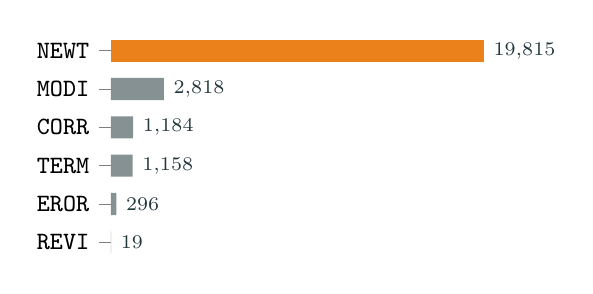
\begin{tikzpicture}
\begin{axis}[xbar, width=7.2cm, height=4.6cm, bar width=8pt,
  xmin=0, xmax=23500, axis x line=none, axis y line*=left, y axis line style={draw=none},
  symbolic y coords={REVI,EROR,TERM,CORR,MODI,NEWT}, ytick={REVI,EROR,TERM,CORR,MODI,NEWT},
  yticklabel style={font=\ttfamily\small}, enlarge y limits=0.12,
  nodes near coords, nodes near coords style={font=\scriptsize},
  nodes near coords style={font=\scriptsize,text=ink}]
\addplot[fill=ink!55, draw=none, bar shift=0pt] coordinates {(19,REVI) (296,EROR) (1158,TERM) (1184,CORR) (2818,MODI)};
\addplot[fill=accent, draw=none, bar shift=0pt] coordinates {(19815,NEWT)};
\end{axis}
\end{tikzpicture}
\end{column}
\begin{column}{0.44\textwidth}
\begin{alertblock}{같은 거래가 여러 행}
새 거래는 \num{78\%}. 나머지 22\%는 변경·정정·종료·오류.\\
그대로 평균을 내면 \textbf{이중 계산}.
\end{alertblock}
\small
\begin{tabular}{@{}l r@{}}
블록 거래 & 1,925 \\
원금 상한 \texttt{+} & 1,556 \\
청산 예정 / 비청산 & 20,026 / 5,206 \\
원화 CD 91D & 약 275 \\
\end{tabular}
\end{column}
\end{columns}
\end{frame}

\begin{frame}{어느 통화가 많나}
\begin{columns}[c]
\begin{column}{0.58\textwidth}
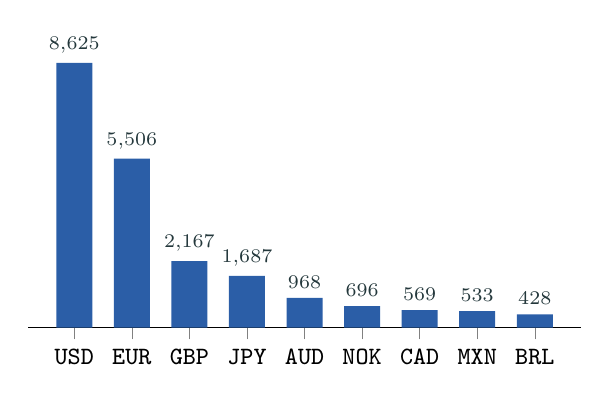
\begin{tikzpicture}
\begin{axis}[ybar, width=8.6cm, height=5.4cm, bar width=13pt,
  ymin=0, ymax=9800, axis y line=none, axis x line*=bottom,
  symbolic x coords={USD,EUR,GBP,JPY,AUD,NOK,CAD,MXN,BRL}, xtick=data,
  xticklabel style={font=\ttfamily\small},
  nodes near coords, nodes near coords style={font=\scriptsize},
  nodes near coords style={text=ink}]
\addplot[fill=blue, draw=none] coordinates {(USD,8625) (EUR,5506) (GBP,2167) (JPY,1687) (AUD,968) (NOK,696) (CAD,569) (MXN,533) (BRL,428)};
\end{axis}
\end{tikzpicture}
\end{column}
\begin{column}{0.38\textwidth}
\small
\begin{block}{기초금리 상위}
\texttt{USD-SOFR-OIS} 3,375\\
\texttt{USD-SOFR} 2,824\\
\texttt{EUR-EURIBOR} 2,152\\
\texttt{GBP-SONIA} 944
\end{block}
\src{통화 = Notional currency-Leg 1. 달러가 34\%.}
\end{column}
\end{columns}
\end{frame}

\begin{frame}{체결에서 공개까지 걸린 시간}
\begin{columns}[c]
\begin{column}{0.55\textwidth}
\begin{tikzpicture}[x=0.82cm]
\draw[line width=1.2pt,ink] (0,0) -- (9,0);
\foreach \x/\l in {0/체결, 1.2/1.7분, 4/15분, 8.6/며칠}
  \draw[ink] (\x,0.12) -- (\x,-0.12) node[below,font=\scriptsize] {\l};
\node[circle,fill=accent,inner sep=3pt] at (1.2,0) {};
\node[above=4pt,font=\small\bfseries,accent] at (1.2,0) {보통 거래};
\node[circle,fill=blue,inner sep=3pt] at (4,0) {};
\node[above=4pt,font=\small\bfseries,blue] at (4,0) {블록 거래};
\node[circle,fill=muted,inner sep=3pt] at (8.6,0) {};
\node[above=4pt,font=\small\bfseries,muted] at (8.6,0) {늦은 신고};
\end{tikzpicture}
\end{column}
\begin{column}{0.40\textwidth}
\small
\begin{block}{측정}
2026-11-27 아침 최근 거래 100건\\
\texttt{executionTimestamp} →\\ \texttt{disseminationTimestamp}
\end{block}
\begin{itemize}\setlength\itemsep{2pt}
\item 중앙값 \num{1.7분}
\item 블록 거래 \num{약 15분}
\item 옛 거래의 변경은 며칠 뒤
\end{itemize}
\end{column}
\end{columns}
\end{frame}

% ─────────────────────────────────────────────
\section{네 곳이 어떻게 이어지나}

\begin{frame}{하루짜리 금리에서 30년 금리까지}
\begin{columns}[c]
\begin{column}{0.36\textwidth}
\begin{tikzpicture}
\node[box=blue] (s) {② SOFR · 하루};
\node[box=accent,below=0.55cm of s] (w) {① SOFR 스왑 · 1–30년};
\node[box=teal,below=0.55cm of w] (t) {③ 국채 곡선 · 1개월–30년};
\node[box=ink,below=0.55cm of t] (a) {④ 국채 경매 낙찰 금리};
\draw[arr] (s) -- node[right,font=\scriptsize,text width=3cm]{앞으로 평균 SOFR는?} (w);
\draw[arr,<->] (w) -- node[right,font=\scriptsize\bfseries,accent]{스왑 스프레드} (t);
\draw[arr] (a) -- (t);
\end{tikzpicture}
\end{column}
\begin{column}{0.62\textwidth}
\centering
\begin{tikzpicture}
\begin{axis}[width=9.4cm, height=5.2cm, xmode=log, log basis x=10,
  xtick={0.003,0.083,1,5,10,30}, xticklabels={1일,1개월,1년,5년,10년,30년},
  xticklabel style={font=\scriptsize}, yticklabel style={font=\scriptsize},
  ylabel={\%}, ylabel style={font=\scriptsize}, ymin=3.8, ymax=5.4,
  grid=major, grid style={soft!60!muted!25},
  legend style={font=\scriptsize,draw=none,at={(0.5,-0.18)},anchor=north,legend columns=2,/tikz/every even column/.append style={column sep=8pt}}]
\addplot[teal, line width=1.3pt, mark=*, mark size=1.4pt] coordinates {
 (0.083,4.27) (0.25,4.34) (0.5,4.44) (1,4.56) (2,4.61) (3,4.64) (5,4.65) (7,4.74) (10,4.85) (20,5.28) (30,5.24)};
\addlegendentry{③ 국채 (11/25)}
\addplot[accent, line width=1.3pt, mark=square*, mark size=1.5pt] coordinates {
 (1,4.512) (2,4.459) (3,4.385) (5,4.344) (7,4.361) (10,4.435) (20,4.625) (30,4.572)};
\addlegendentry{① SOFR 스왑 중앙값 (11/25)}
\addplot[blue, only marks, mark=diamond*, mark size=3pt] coordinates {(0.003,3.94)};
\addlegendentry{② SOFR (11/24)}
\addplot[ink, only marks, mark=triangle*, mark size=3pt] coordinates {(0.077,4.115)};
\addlegendentry{④ 4주 단기채 낙찰 (11/25)}
\end{axis}
\end{tikzpicture}\\
\src{① 11/25 바로 시작한 SOFR 스왑 신규 거래 1,142건, 만기별 고정금리 중앙값. 실습 D에서 직접 만든다.}
\end{column}
\end{columns}
\end{frame}

\begin{frame}{스왑 스프레드 = SOFR 스왑 – 국채 \src{\normalsize 2026-11-25}}
\begin{columns}[c]
\begin{column}{0.55\textwidth}
\begin{tikzpicture}
\begin{axis}[ybar, width=8.2cm, height=5.2cm, bar width=14pt,
  ymin=-75, ymax=5, axis x line*=top, axis y line=none,
  symbolic x coords={1년,2년,3년,5년,7년,10년,20년,30년}, xtick=data,
  xticklabel style={font=\small},
  nodes near coords, nodes near coords style={font=\scriptsize,anchor=north},
  nodes near coords style={text=ink}]
\addplot[fill=accent, draw=none] coordinates {(1년,-4.8) (2년,-15.1) (3년,-25.5) (5년,-30.6) (7년,-37.9) (10년,-41.5) (20년,-65.5) (30년,-66.8)};
\end{axis}
\end{tikzpicture}\\
\src{단위: bp (0.01\%p)}
\end{column}
\begin{column}{0.42\textwidth}
\begin{block}{생각해 볼 것}
만기가 길수록 스왑 금리가 국채보다 \textbf{더 낮다}.\\[3pt]
정부가 빌리는 값보다 은행 간 금리 약속이 싸다?
\end{block}
\begin{alertblock}{1일차와 연결}
구조화상품의 \textbf{추정가치}를 계산할 때 쓰는 할인율이 이 근처에서 나온다.
\end{alertblock}
\end{column}
\end{columns}
\end{frame}

% ─────────────────────────────────────────────
\section{실습}

\begin{frame}[fragile]{Claude에게 네 곳에서 한 건씩 받아 오게 하기 \src{\normalsize 7분}}
\begin{block}{Claude Code 패널에 붙여 넣기 \src{(전문은 실습지 5절)}}
\scriptsize
아래 네 곳에서 각각 가장 최근 값 한 건씩만 받아서 표로 보여줘. 짧은 코드는 \texttt{jpm\_kit/out/}에 파일로 만들어 \texttt{uv run}으로 실행해.\\
1. DTCC 최근 금리 스왑 거래 — 원화(KRW) 거래가 있으면 그것\\
2. NY Fed SOFR \quad 3. 재무부 국채 수익률 곡선 (1·2·5·10·30년) \quad 4. TreasuryDirect 최근 경매\\
규칙: 각 주소에 한 번씩만, 실패하면 다시 시도하지 말 것. HTTP 요청은 \texttt{urllib} 말고 \alert{\texttt{httpx}}로.\\
마지막에 "체결/기준 시각"이 서로 얼마나 다른지 한 줄로.
\end{block}
\small
\begin{columns}[T]
\begin{column}{0.48\textwidth}
\textbf{적을 것}
\begin{itemize}\setlength\itemsep{1pt}
\item DTCC 거래: 통화 / 만기 / 고정금리
\item 체결 → 공개 걸린 시간
\item SOFR, 국채 10년, 최근 경매
\end{itemize}
\end{column}
\begin{column}{0.48\textwidth}
\textbf{리허설 결과} \src{(11/27, 약 100초)}
\begin{itemize}\setlength\itemsep{1pt}
\item 원화 5년 CD 스왑 3.57\%, 공개까지 1분 18초
\item 국채 11/25, SOFR 11/24 — \alert{최대 사흘 차이}
\end{itemize}
\end{column}
\end{columns}
\end{frame}

\begin{frame}{확인 질문}
\begin{enumerate}\setlength\itemsep{10pt}
\item DTCC 하루치 파일에서 고정금리 평균을 바로 내면 \textbf{어떤 행} 때문에 틀어질까?
\item 원금 칸이 \texttt{250,000,000+}인 거래가 많은 날, ``그날 원금 합계''는 실제보다 큰가, 작은가?
\item JPMorgan이 낸 스왑 거래만 골라낼 수 있나? 없다면 왜?
\item SOFR(하루)와 10년 SOFR 스왑 금리는 왜 다를까?
\end{enumerate}
\end{frame}

\begin{frame}{이용 규칙}
\begin{itemize}\setlength\itemsep{8pt}
\item \textbf{DTCC 주소는 공식 API가 아니다.} 공개 대시보드가 쓰는 주소라 바뀔 수 있다. 같은 주소를 1분에 한 번 이하로 부르고, 많이 받을 때는 하루치 zip.
\item \textbf{출처를 밝힌다}: DTCC Public Price Dissemination · Federal Reserve Bank of New York · U.S.\ Department of the Treasury.
\item \textbf{\texttt{httpx}를 쓴다.} 파이썬 기본 \texttt{urllib}은 TreasuryDirect 인증서를 확인하지 못한다 (\texttt{CERTIFICATE\_VERIFY\_FAILED}).
\item 재무부 Fiscal Data API는 교내 네트워크에서 막힐 수 있어 오늘은 쓰지 않는다.
\end{itemize}
\end{frame}

\end{document}
